\documentclass[12pt]{article}

\title{LaTeX Cheatsheet}
\author{author name}
% If commented out, uses today's date
%\date{01/01/2000}

\usepackage{shared}

% Set margins.
%\usepackage[top=2in, bottom=1.5in, left=1in, right=1in]{geometry}
% Set all margins to the same value
%\usepackage[margin=1in]{geometry}

\usepackage{boxedminipage}
% A5 output. You should use this always for e-reader users who have small screens.
\usepackage[a4paper]{geometry}
\usepackage{pdfpages}
% Show labels. Use labels with at most 7 chars or you fall off PDF in A5 kindle friendly mode.
\usepackage[notref,notcite]{showkeys}
% Break line inside table cell: http://tex.stackexchange.com/questions/2441/how-to-add-a-forced-line-break-inside-a-table-cell
\usepackage{tabularx}
  % TODO get centering working
  %\usepackage{ragged2e}       % Center all tabularx: http://tex.stackexchange.com/questions/89166/centering-in-tabularx-and-x-columns
  %\renewcommand\tabularxcolumn[1]{>{\Centering}p{#1}}
\usepackage{wrapfig}

% TODO can this work? Print both verbatim and code?
% CANT use verbatim here, give up, people will read at source for now!
%\newcommand{\inOut}[1]{\begin{verbatim}#1\end{verbatim}#1}
% Dummy `inOut` before I can find a nice way to show source and output in one go.
\newcommand{\inOut}[1]{#1}

\begin{document}

\tableofcontents
\newpage

%\begin{comment}
\section{TODO}

\begin{remark}
Put TODOs as the first \label{TODO2} thing for development so you don't forget to do them.

You may want to put those in order of urgency/difficulty here.

Mark TODO location in \label{TODO1} the middle of text with labels TODO, then explain them here.

Comment them out for release.
\end{remark}

\begin{itemize}
\item TODO2 deal with this TODO at all costs
\item TODO1 this TODO is not as important as the first one.
\item TODO3
\end{itemize}
%\begin{comment}

\section{Title pages} \label{title-pages}

\maketitle
\newpage

%#complex title page
\begin{titlepage}
COMPLEX TITLE PAGE

PROMOTION 2009

DURAN SANTILLI Ciro

\vspace{40 mm}

\begin{center}

{\large RAPPORT DE STAGE DE RECHERCHE}\\[0.5cm]

\underline{ \large \bfseries \itshape Flatness in control systems}

\vspace{10 mm}

\underline{ \bfseries NON CONFIDENTIEL }

PUBLICATION

\end{center}

\vspace{40 mm}

\underline{Option} : Mathématiques apliquées

\underline{Champ de l'option} : Automatique et Contrôle

\vspace{5 mm}

INRIA Sophia Antipolis Méditerrané

2004 Route des Lucioles - BP93

06902 SOPHIA ANTIPOLIS Cedex France
\end{titlepage}

\newpage

\section{Abstract} \label{abstract}

\begin{abstract}
This attempts to cover every single feature of LaTeX to its minute details.

It is intended to work with the \href{https://www.tug.org/texlive/acquire-iso.html}{TeX Live 2013 full ISO} without any additional packages installed or updated.
\end{abstract}
\newpage

\section{Special Characters}

The following 10 special chars have to be escaped because they have a special meaning in TeX.

All of them can be escaped with \lstinline|verb|, and many, but not all can be escaped with the backslash. Some have a special macro for them.

In short, pure insanity!

\begin{itemize}
\item dollar sign

Backslash: \$

\item underscore:

Verb: \verb|a_b|.

Backslash: a\_b

TODO what is the TeX function?

\item sharp / hash / number sign:

Verb: \verb|#|.

Backslash: \#

Used for macro parameters.

\item tilde:

\url{http://tex.stackexchange.com/questions/9363/how-does-one-insert-a-backslash-or-a-tilde-into-latex}

Center the tilde vertically: \url{http://tex.stackexchange.com/questions/312/correctly-typesetting-a-tilde}

\lstinline|\textasciitilde|: \textasciitilde

Verb: \verb|~|

Unescaped is a NBSP.

Without tilde:

mmmmmmmmmmmmmmmmmmmmmmmmmmmmmmmmmmmmmmmmmmmmmmmmmm nnnnnnnnnnnnnnnnnnnnnnnnnnnnnnnnnnnnnnnnnnnnnnnnnn 

With tilde:

mmmmmmmmmmmmmmmmmmmmmmmmmmmmmmmmmmmmmmmmmmmmmmmmmm~nnnnnnnnnnnnnnnnnnnnnnnnnnnnnnnnnnnnnnnnnnnnnnnnnn 

Recommended before \lstinline|\ref| and object type: \lstinline|Table\ref{tab1}|.
\end{itemize}

\section{Symbols}\label{symbols}

To find a symbol for which you do not know the name,
consider using a character recognition service like \url{http://detexify.kirelabs.org/classify.html}.
Backend source at: \url{https://github.com/kirel/detexify-hs-backend}.

\begin{itemize}
\item ellipsis:

\begin{itemize}
\item  \ldots   - horizontally at bottom of line
\item  $\cdots$ - horizontally center of line (math mode only)
\item  $\ddots$ - diagonal (math mode only)
\item  $\vdots$ - vertical (math mode only)
\end{itemize}

\item international:

With \lstinline|\usepackage[utf8]{inputenc}|:

á à â ä

Chinese does not work: %中文

\item Derivatives:

$$ \frac{dx(t)}{dt} $$
$$ \frac{\partial x(u,v)}{\partial u} $$

\item Vector arrow: $\vec{F}$

\item Arrow with text above from amsmath:

$A\xrightarrow{x^2}B$

Arrow text above and below. \href{http://tex.stackexchange.com/questions/27545/custom-length-arrows-text-over-and-under}{Seems not to be on any package}:

$A\xxrightarrow{x^1}[x^2]{x^3}B$

$A\xxrightarrow{1000}{1}A$

\item TeX and LaTeX logos. Good for tests: \TeX\ \LaTeX
\end{itemize}

\section{Font}\label{font}

\begin{itemize}
\item {\Large Large brackets}
\item
\begin{Large}begin large environment\end{Large}
{\Large large inside brackets}
Possible sizes:
\begin{lstlisting}
\tiny
\scriptsize
\footnotesize
\small
\normalsize
\large
\Large
\LARGE
\huge
\Huge
\end{lstlisting}

Arbitrary sizes are only possible for Type 1 fonts: \url{http://stackoverflow.com/questions/890127/how-to-set-latex-font-size-in-millimeter}
\url{http://en.wikipedia.org/wiki/PostScript_fonts#Font_type}
\item \textbf{textbf command}
\item {\bf bf brackets bold}
\item \textit{textit command}
\item {\it it}
\item {\it \bf it bf}
\item {\bf \it bf it}
\item \underline{underline underline}
\item \uline{uline uline}. Requires \lstinline|\usepackage{ulem}|
\end{itemize}

\section{Sections}\label{sections}

\subsection{Subsection}\label{subsection}

\subsubsection{Subsubsection}\label{subsubsection}

\paragraph{Paragraph}\label{paragraph}

Paragraph comes after \lstinline|subsubsection|.

To add a label and numbering to it, use:

\begin{lstlisting}
\setcounter{secnumdepth}{4}
\end{lstlisting}

To add it to the TOC use:

\begin{lstlisting}
\setcounter{tocdepth}{4}
\end{lstlisting}

\subparagraph{Subparagraph}\label{subparagraph}

Subparagraph comes after paragraph.

To add a label and numbering to it, use:

\begin{lstlisting}
\setcounter{secnumdepth}{5}
\end{lstlisting}

To add it to the toc, use:

\begin{lstlisting}
\setcounter{tocdepth}{5}
\end{lstlisting}

\section{Positioning}\label{positioning}

\begin{center}
center environment

center environment
\end{center}

{\centering
centering group

centering group: only works for single paragraphs
}

\begin{flushright}
flushright environment

flushright environment
\end{flushright}

TODO why does it not work?

{\flushright flushright group}

\subsection{Left and right at the same time}

\begin{minipage}[t]{0.5\textwidth}
\flushleft
left1

left2
\end{minipage}
\hfill
\begin{minipage}[t]{0.5\textwidth}
\flushright
right1

right2
\end{minipage}

\subsection{Wrap}\label{wrap}

hfill float right:

left \hfill float right \\
left \hfill float right \\

\begin{boxedminipage}{\textwidth}
Multiple paragraphs

with a border.
\end{boxedminipage}

\section{vspace}\label{wrap}

vspace 1cm

\vspace{1cm}

vspace 1cm \\[1cm]

vspace 1cm

textwidth = width of the page where text can be (no margins)

\subsection{Paragraph indentation}\label{paragraph-indentation}

By default, all paragraphs are indented, except the first one after a section. This is a typographical convention \url{http://tex.stackexchange.com/questions/39227/no-indent-in-the-first-paragraph-in-a-section}.

To also indent the first paragraph after sections, use \lstinline|\usepackage{indentfirst}|.

To remove the indent of all paragraphs, set \lstinline|\setlength{\parindent}{0cm}|. \lstinline|parindent| is a TeX primitive.

To remove the indent of a single paragraph, use:

\begin{lstlisting}
\noindent Paragraph without indent.
\end{lstlisting}

\lstinline|noindent| is a TeX primitive.

\subsection{setlength vs =}\label{setlength-vs-eq}

It is possible to set certain variables either as \lstinline|\parskip=3pt| or \lstinline|\letlength{\parskip}{3pt}|.

The following explains the difference: \url{http://tex.stackexchange.com/questions/6558/what-is-the-right-way-to-set-a-dimension-parameter}

\section{Equations}\label{equations}

\section{Formulas}\label{formulas}

Most of low level formula stuff is present in \TeX and shall not be discussed here.

\LaTeX\ style inline \(x^2\) equation.

\LaTeX\ style displayed equation:

\[ x^2 \]

Unnumbered equation:

\begin{equation*}
\dot{x} = f(x,u)
\end{equation*}

Numbered formula:

\begin{equation}\begin{aligned}\label{eqFor1}
\dot{x} = f(x,u)
\end{aligned}\end{equation}

Align at multiple points:

\begin{alignat*}{3}
& a + b && = c   && = c2 \\
& d   && = e + f && = f2
\end{alignat*}

\begin{remark}\label{remFor1} Why I use equation + aligned by default
There are simpler ways to write the equation such as backslash square brackets \textbackslash{}[\ldots\textbackslash{}], but if you use those you will soon notice that you will waste a long time modifying equations either to make them multiline, or to give them numbers, so it is just better to always use equation + aligned unless you have a reason not to do so.
\end{remark}

Case function definition:

\begin{equation}
f(x) =
\begin{cases}
x & x \le 0 \\
-x & x>0
\end{cases}
\end{equation}

\section{Floats}\label{floats}

Floats are objects like tables or images that cannot be split across pages. Therefore, they may be displaced by LaTeX which can put text before them to not leave empty space.

Since floats may have floated around, always refer to them via reference label pairs, like Float~\ref{float1}, \emph{never} as ``The next float''.

\begin{table}
\begin{tabular}{cc}
1 \\ 1 \\ 1 \\ 1 \\ 1 \\
\end{tabular}
\caption{float1}
\label{float1}
\end{table}

Don't worry too much about float positioning in early development: only think about it when you are almost done and the document won't be changing too much.

Different options can increase the probability that floats won't float around too much. It may be a good idea to initially develop with \lstinline|[!htbp]| to see text close to floats and only remove it latter if needed. Table~\ref{floatHtpb} uses those options.

\begin{table}
\begin{tabular}{cc}
!htbp \\ !htbp \\ !htbp \\ !htbp \\ !htbp \\
\end{tabular}
\caption{floatHtpb}
\label{floatHtpb}
\end{table}

The float package offers the option \lstinline|H| which fixes the float at a position without reflow no matter what.

TODO, what does each character mean exactly?

\begin{itemize}
\item \lstinline|!|
\item \lstinline|h|
\item \lstinline|t|
\item \lstinline|b|
\item \lstinline|p|
\end{itemize}

SE thread: \url{http://tex.stackexchange.com/questions/2275/keeping-tables-figures-close-to-where-they-are-mentioned}

\section{Figures}\label{figures}

Figures, images, graphics.

See Figure~\ref{fig-label}.

\begin{figure}[htb]
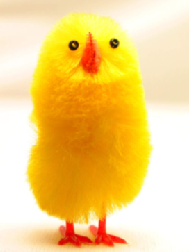
\includegraphics[width=5cm]{image.png}
\caption{caption here}
\label{fig-label}
\end{figure}

Allowed formats:

\begin{itemize}
\item PNG
\item JPG
\end{itemize}

Non-allowed formats:

\begin{itemize}
\item GIF
\end{itemize}

You can append to the figure search path with the package \lstinline|graphicx| and the command \lstinline|\graphicspath|:

\begin{lstlisting}
\usepackage{graphicx}

\graphicspath{{./media/}{/usr/share/latex/img/}}
\end{lstlisting}

Relative paths are taken relative to current directory.

You can only use the \lstinline|\graphicspath| command once! Newer calls will erase the older ones.

%  Test media-gen:
%
%    \begin{figure}[htb]
%      \includegraphics[width=5cm]{media-gen.png}
%      \caption{caption here}
%      \label{fig-label}
%    \end{figure}

\subsection{wrapfigure}\label{wrapfigure}%#float images

wrapfigure from wrapfig package allows images to float right around text.
Images float only around text that comes after them.

a \\ a \\ a \\ a\\ a \\ a \\ a \\ a \\ a\\ a \\

\begin{wrapfigure}{r}{0.5\textwidth}
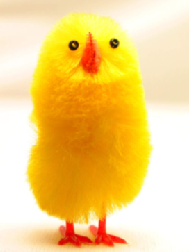
\includegraphics[height=2cm]{image.png}
\caption{Floating chick B}
\end{wrapfigure}

b \\ b \\ b \\ b\\ b \\ b \\ b \\ b \\ b\\ b \\
b \\ b \\ b \\ b\\ b \\ b \\ b \\ b \\ b\\ b \\

\begin{wrapfigure}{r}{0.5\textwidth}
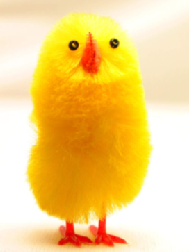
\includegraphics[height=2cm]{image.png}
\caption{Floating chick C}
\end{wrapfigure}

c \\ c \\ c \\ c\\ c \\ c \\ c \\ c \\ c\\ c \\
c \\ c \\ c \\ c\\ c \\ c \\ c \\ c \\ c\\ c \\

\begin{wrapfigure}{l}{0.5\textwidth}
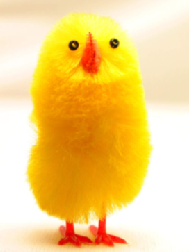
\includegraphics[height=2cm]{image.png}
\caption{Floating chick D}
\end{wrapfigure}

d \\ d \\ d \\ d\\ d \\ d \\ d \\ d \\ d\\ d \\
d \\ d \\ d \\ d\\ d \\ d \\ d \\ d \\ d\\ d \\

\begin{wrapfigure}{r}{5cm}
\begin{flushleft}
Floating

Paragraphs

E
\end{flushleft}
\end{wrapfigure}

TODO: how to remove top margin?

e \\ e \\ e \\ e\\ e \\ e \\ e \\ e \\ e\\ e \\
e \\ e \\ e \\ e\\ e \\ e \\ e \\ e \\ e\\ e \\

Does not work one to left one to right:

\begin{wrapfigure}{l}{0.3\textwidth}
Floating

Paragraphs

l
\end{wrapfigure}

\begin{wrapfigure}{r}{0.5\textwidth}
Floating

Paragraphs

r
\end{wrapfigure}

\clearpage

\section{Tables}\label{table}

Table~\ref{table1} is a simple table.

\begin{table}
\begin{tabular}{ccc}
h1 & h2 & h3 \\
\hline
1 & 2 & 3 \\
4 & 5 & 6 \\
7 & 8 & 9 \\
\end{tabular}
\caption{table1}
\label{table1}
\end{table}

For complex tables with label \lstinline|LABEL|, create a \lstinline|LABEL.ods| spreadsheet with same name as the label and use it to make the table, then copy paste to the TeX.

As with any other float (object that can change its position on the page to fit to content), always reference table labels when talking about tables, and never use expressions such as "the table" or "next table".

Table~\ref{table-format} shows how to format individual table columns with \lstinline|\usepackage{array}|.

\begin{table}
\begin{tabular}{l c rp{1cm} p{1cm} >{\bf}c >{\it}c | c || c @{abc} c c}
1 & 2 & 3 & 4 & 5 5 5 5 5 & 6 & 7 & 8 & 9 & 10 & 111111111111111111111111111111111111111111111 \\
1 & 2 & 3 & 4 & 5 5 5 5 5 & 6 & 7 & 8 & 9 & 10 & 111111111111111111111111111111111111111111111 \\
\end{tabular}
\caption{table-format}
\label{table-format}
\end{table}

\subsection{Header}\label{table-header}

There is no default semantic macro for the header like in HTML: people usually simply define inline styles. But that can only be done for an entire row with \lstinline|tabu| + \lstinline|rowfont| and not with \lstinline|tabular|. This is so horrendous that I'd rather not have the header, or at most just an \lstinline|hline| as in table~\ref{table-header-hline}.

\begin{table}
\begin{tabular}{ll}
a & b \\
\hline
1 & 2 \\
3 & 4
\end{tabular}
\caption{table-format}
\label{table-header-hline}
\end{table}

\subsection{Avoid specifying column specifiers}\label{table-header}

TODO how to avoid specifying the column specifiers. It is not DRY since it repeats the number of column information, and it is style instead of semantics.

Seems not possible neatly: \url{http://tex.stackexchange.com/questions/188589/table-without-column-specification}.

Best workaround: specify a large number of columns as in Table~\ref{tab-no-specifier}.

\begin{table}
\begin{tabular}{*{9}{l}}
a & b \\
\hline
1 & 2 \\
3 & 4
\end{tabular}
\caption{Table without column specifiers in source.}
\label{tab-no-specifier}
\end{table}

\subsection{Break line inside table cell}\label{break-line-inside-table-cell}

SE question: \url{http://tex.stackexchange.com/questions/2441/how-to-add-a-forced-line-break-inside-a-table-cell}

The best solution we have found so far it is to use \lstinline|tabularx| and \lstinline|\newline|. as in Table~\ref{table-break-tabularx}. \emph{Warning}: for \lstinline|tabularx| to work, you \emph{must} have an \lstinline|X| column!

\begin{table}[!htpb]
\begin{tabularx}{\textwidth}{lX}
a & a \newline
    b \\
a & a \newline
    b \\
\end{tabularx}
\caption{table-break-tabularx}
\label{table-break-tabularx}
\end{table}

TODO how to get it automatically centered? floatrow does not work on it: \url{http://tex.stackexchange.com/questions/89166/centering-in-tabularx-and-x-columns}

Table~\ref{table-break} shows how to format individual table columns without any extra packages:

\begin{table}[!htpb]
\begin{tabular}{l l}
a & \begin{tabular}[t]{@{}l@{}} a \\ b \end{tabular} \\
\hline
a & \begin{tabular}[c]{@{}l@{}} a \\ b \end{tabular} \\
\hline
a & \begin{tabular}[b]{@{}l@{}} a \\ b \end{tabular} \\
\hline
\end{tabular}
\caption{table-break}
\label{table-break}
\end{table}

\subsection{Fixed width cell}\label{fixed-width-cell}

\begin{tabular}{>{}m{10cm} | l}
10cm default align & col2
\end{tabular}

\begin{tabular}{>{\centering}m{10cm} | l}
10cm center & col2
\end{tabular}

\begin{tabular}{>{}m{10cm} | l}
10cm center & col2
\end{tabular}

\section{Include external TeX files}\label{include}

There are two \LaTeX\ commands that achieve this effect: \lstinline|include| and \lstinline|input|.

\lstinline|input| is a \TeX\ primitive, \lstinline|include| not.

Difference: \url{http://tex.stackexchange.com/questions/246/when-should-i-use-input-vs-include}.

There seems to be no neat way to include an entire directory or use wildcards \url{http://tex.stackexchange.com/questions/13921/inputting-multiple-files-in-latex}

\section{Include external PDF}\label{include-external-pdf}

The following page shall be taken from an external PDF:


\includepdf[pagecommand=\thispagestyle{plain}]{image.pdf}

TODO: how to show the page number and make a label / hyperref to it? <http://tex.stackexchange.com/questions/25105/unable-to-link-to-inserted-pages-with-pdfpages>

\section{Comments}\label{comments}

Next line will be commented out, and therefore invisible to output.
\begin{comment}
This line was commented off.
\end{comment}

\section{Verbatim}\label{verbatim}

Regular text.

Block:

\begin{verbatim}
a
  b
c
\end{verbatim}

Inline \verb|~| tilde.

There is no way to indent verbatim relative to its containing environment, but it can be done with \lstinline|lstlisting|. \url{http://tex.stackexchange.com/questions/164993/indent-content-of-verbatim-lstlisting-environment-relative-to-containing-envir#164999}

\section{Computer code listings}\label{computer-code}

Use \lstinline|\usepackage{lstlisting}|

This is how you use it:

\begin{lstlisting}
if i in is:
    echo i
else:
    echo -i
\end{lstlisting}

Inline listings: \lstinline|func_f(void a)| is a function.

Set the language: TODO not highlighting. Why?

\begin{lstlisting}[language=Python]
def f(x):
    return x + 1
\end{lstlisting}

\begin{lstlisting}[language=Ruby]
def f(x)
  x + 1
end
\end{lstlisting}

Set up a caption and label. See Listing~\ref{listing}.

\begin{lstlisting}[label=listing, caption={Listing with caption and label.}]
def f(x):
  return x + 1
\end{lstlisting}

Frame the code listing with a surrounding box: \url{http://tex.stackexchange.com/questions/14967/source-code-listing-with-frame-around-code}

You can set properties for the entire document by using \lstinline|lstset| in the header:

\begin{lstlisting}
  \lstset{
    %language=C,                             % Code langugage
    basicstyle=\ttfamily,                    % Code font, Examples.
    %commentstyle=\color{gray},              % Comments font
    %numbers=left,                           % Line nums position
    %numberstyle=\tiny,                      % Line-numbers fonts
    %stepnumber=1,                           % Step between two line-numbers
    %numbersep=5pt,                          % How far are line-numbers from code
    %backgroundcolor=\color{lightlightgray}, % Choose background color
    %frame=none,                             % A frame around the code
    %tabsize=4,                              % Default tab size
    %captionpos=b,                           % Caption-position = bottom
    %breaklines=true,                        % Automatic line breaking?
    %breakatwhitespace=false,                % Automatic breaks only at whitespace?
    %showspaces=false,                       % Dont make spaces visible
    %showtabs=false,                         % Dont make tabls visible
    %columns=flexible,                       % Column format
    %keywordstyle=\color{OliveGreen},        % Keywords font ('*' = uppercase)
    %morekeywords={__global__, __device__},  % CUDA specific keywords
  }
\end{lstlisting}

Bad defaults which you should correct are:

\begin{itemize}
\item
Use the package \lstinline|upquote| so that quotation marks will appear
correctly as ASCII characters: \lstinline|"'`|.
\item
Use the option \lstinline|basicstyle=\ttfamily| allows outputs monospace fonts:
\begin{lstlisting}
mmmmmmmmm
iiiiiiiii
\end{lstlisting}
\item
Use the \lstinline|literate={~} {$\sim$}{1}| option so that ASCII tildes can be used. \url{http://tex.stackexchange.com/questions/17266/how-to-insert-a-nice-tilde-in-a-lstlisting}.
\item TODO how to copy paste correct code from PDF? paste is always full of spaces.
\end{itemize}

\section{References}\label{references}

\lstinline|\label| refers to the smallest surrounding thing that is numbered, typically a section or a theorem environment. Therefore, if you simply put a label in a point paragraph, you don't normally get a link to that point of paragraph like you would in an HTML anchor.

For HTML ID compatibility, use hyphen separation: def-a-definition-was-here.

\begin{example}\label{expRef1}
The next ref aims at the current example: \ref{expRef1}.
\end{example}

It is a good idea not to leave spaces between \lstinline|labels|.

The floatrow package is a must: \lstinline|\usepackage{floatrow}| automatically centers all floats.

\section{Hyperlinks and URLs}\label{hyperlinks-urls}

External links:

\url{http://example.com}

\href{http://example.com}{example.com}

Relative links:

\url{./index.pdf}

\href{./index.pdf}{Link to index.pdf.}

\lstinline|url| and \lstinline|href| with special characters like hash \# without escaping it: \url{http://example.com?a=b&c=d#id}, \href{http://example.com?a=b&c=d#id}{href to http://example.com\#id}. In \lstinline|href| works fine for the URL, but fails for the link text, as expected.

\href{./index.pdf}{Link to index.pdf.}

Inner links in document with \lstinline|hypertarget| + \lstinline|hyperlink|:

\hypertarget{label}{target caption}

\hyperlink{label}{link caption}

\section{Variables, conditionals}\label{variables}

Possible with \lstinline|if| and \lstinline|def|. Both are \TeX\ primitives and shall not be commented here.

You should never use those things on your \LaTeX\ documents: leave them for insane package writers.

\section{Quotations}\label{quotations}

From \cite{Aa00}:

\begin{quote}
Some quoted text, single paragraph. Some quoted text, single paragraph. Some quoted text, single paragraph.
Some quoted text, single paragraph. Some quoted text, single paragraph. Some quoted text, single paragraph.
Some quoted text, single paragraph. Some quoted text, single paragraph. Some quoted text, single paragraph.
Some quoted text, single paragraph. Some quoted text, single paragraph. Some quoted text, single paragraph.
Some quoted text, single paragraph. Some quoted text, single paragraph. Some quoted text, single paragraph.
Some quoted text, single paragraph. Some quoted text, single paragraph. Some quoted text, single paragraph.
Some quoted text, single paragraph. Some quoted text, single paragraph. Some quoted text, single paragraph.
\end{quote}

Quotations: for use with longer quotations, of more than one paragraph, because it indents the first line of each paragraph.

Verse: is for quotations where line breaks are important, such as poetry. Once in, new stanzas are created with a blank line, and new lines within a stanza are indicated using the newline command.

If a line takes up more than one line on the page, then all subsequent lines are indented until explicitly separated with \lstinline|\\|.

\section{Forms}

\begin{Form}[action={http://your-web-server.com/path/receiveform.cgi}]
\begin{tabular}{l}
\TextField{Name} \\
\CheckBox[width=1em]{Check} \\
\Submit{Submit}
\end{tabular}
\end{Form}

\section{Bibliography}

\section{cite}\label{cite}

\LaTeX\ has built-in bibliography capabilities which allow you to write the bibliography inline, but the best way is to use BibTeX because:

\begin{itemize}
\item it separates style from data well: you give the data, and multiple output styles are possible.
\item it is easier to reuse since it is on a separate file (true, you could use \lstinline|input|).
\end{itemize}

Several online sources offer BibTeX items for you to copy and past into your documents, and there are also citation managers which help you find, store and automate the citation process.

BibTeX just generates the LaTeX built-in format from a \lstinline|.bib| file into a \lstinline|.bbl| file and inserts it at the \lstinline|\bibliography{}| macro.

The advantage of BibTeX is that you can separated the bibliography from the document and reuse it more easily.

You have to cite a reference before it appears in the bibliography.

In the bibliography command, use the same name as your \lstinline|.bib| file.

Only items that you explicitly cite will appear on the bibliography by default, so you can use any big \lstinline|bib| file for you project. If you want something to appear on the bibliography without citing it, use \lstinline|\nocite{id}|. For good style, put those commands just before the \lstinline|bibliography| command.

\begin{itemize}
\item Aa00: \cite{Aa00}
\item Aa01: \cite{Aa01}
\end{itemize}

You can specify the style of the bibliography with the \lstinline|\bibliographystyle{}|  command.

The \lstinline|natbib| package comes with several common built-in styles.

\section{Index}\label{index}

\begin{itemize}
\item installed in \lstinline|PATH|: \lstinline|makeindex| program. Comes by default with TeX Live 2013, and gets called automatically by \lstinline|latexmk|.
\item on the preamble: \lstinline|\usepackage{makeidx}| and \lstinline|\makeindex|
\item mention a term on a given position: \lstinline|\index{key}|
\item print the index: \lstinline|\printindex|
\end{itemize}

\index{a}
\index{b}

\printindex

\section{Bibliography}\label{secBib}

\bibliographystyle{plain}
\bibliography{main}
\end{document}
